\documentclass{article}

\usepackage{repsty}
\usepackage{wrapfig}

\usepgfplotslibrary{fillbetween}


\begin{document}
The questions are:
\begin{enumerate}
	\item How long to measure the signal?
	\item How many measurements per event are optimal?
	\item How congregated about the zero-crossings the measurements should be?
\end{enumerate}

The analytical expression of the variance of the estimate is\footnote{This expression consistently overestimates the standard error by a factor of 2; however, when used on a function with $x_i = (N_0P)^2$ (linear regression), it yields the same expression as the fitter. The fitter also computes the standard error according to some formula. As far as I can tell, the difference between this one and the one the fitter uses (which I haven't seen yet), is the $sum_j x_j$ factor in the denominator.}
\begin{equation}
\begin{cases}
	\var{\hat\omega} &= \sfrac{\nu}{\sum_j x_j\var[w]{t}}, \\
	\var[w]{t} &= \sum_i w_i \bkt{t_i - \avg{t}_w}^2,~ \avg{t}_w = \sum_i t_i w_i, \\
	w_i &= \frac{x_i}{\sum_j x_j},~ x_i = (N_0P\exp(\lambda t_i))^2\cos^2(\omega t_i + \phi) = \bkt{\mupp}^2.
\end{cases}	
\end{equation}

As one can see, the variance inversely depends on the spread of the predictor variable. This spread is determined mainly by the total duration of measurement, and hence the spin tune decoherence time. Variation in the number of polarimetry measurements per event has only a second-order effect on $\var[w]{t}$.

The two questions that follow both condition the measurement distribution across time. The number of measurements per event determine, with regard to this statistical aspect, the number of events per second, and hence the number of events that can fit within a compaction region. If that number is large, there will be fewer (but more precise) measurements within the high-information regions, and we will have to increase the compaction factor in order to collect enough events, at which point our use of the beam is sub-optimal.

\section{Number of measurements per observation (event)}
\newcommand{\obs}{\epsilon}
\newcommand{\meas}{m}
\newcommand{\Nmo}{n_{\sfrac{\meas}{\obs}}}
\newcommand{\Nozc}{n_{\sfrac{\obs}{zc}}}
\newcommand{\Nzc}{n_{zc}}
\newcommand{\No}{n_{\obs}}

Define the following variables: \begin{inparaenum}[\itshape a\upshape)]
	\item the number of measurements per observation: $\Nmo$;
	\item the number of observations per zero-crossing: $\Nozc$;
	\item the number of zero-crossings per experiment: $\Nzc$.
\end{inparaenum}

The expected total number of scatterings in an experiment with a given number of zero-crossings: $n_m = \underbrace{\Nzc\cdot\Nozc}_{\No}\cdot\Nmo$. ($\No$ is the total number of observations.)

\begin{equation}
\begin{cases}
	\SE{\hat{\omega}}^2 &= \frac{\SE{\obs}^2}{X_{tot}\cdot\sum_{j=1}^{\No}w_j\bkt{t_j - \avg{t}_w}^2}, \\
	\SE{\obs}^2 &= \frac{\SE{\meas}^2}{\Nmo} ,\\
	X_{tot} &= \sum_{j=1}^{\No} x_j = \sum_{s=1}^{\Nzc}\sum_{j=1}^{\Nozc} x_{js}.
\end{cases}
\end{equation}

We can express $\sum_{j=1}^{\Nozc} x_{js} = \Nozc \cdot x_{0s}$, for some mean value $x_{0s}$ in the given zero-crossing $s$. The sum $\sum_{j=1}^{\Nozc} x_{js}$ falls exponentially due to decoherence, hence $x_{0s} = x_{01}\exp{(\lambda\cdot \frac{(s-1)\cdot\pi - \phi}{\omega})}$. Therefore,
\[
	X_{tot} = \Nozc\cdot x_{01} \cdot \frac{\exp{\bkt{\frac{\lambda\phi}{\omega}}}\cdot\bkt*{\exp{\bkt{\frac{\lambda\pi}{\omega}\Nzc}}-1}}{\exp{\bkt{\frac{\lambda\pi}{\omega}}}-1} \equiv \Nozc \cdot g(\Nzc).
\]

\begin{figure}[h]
	\centering
	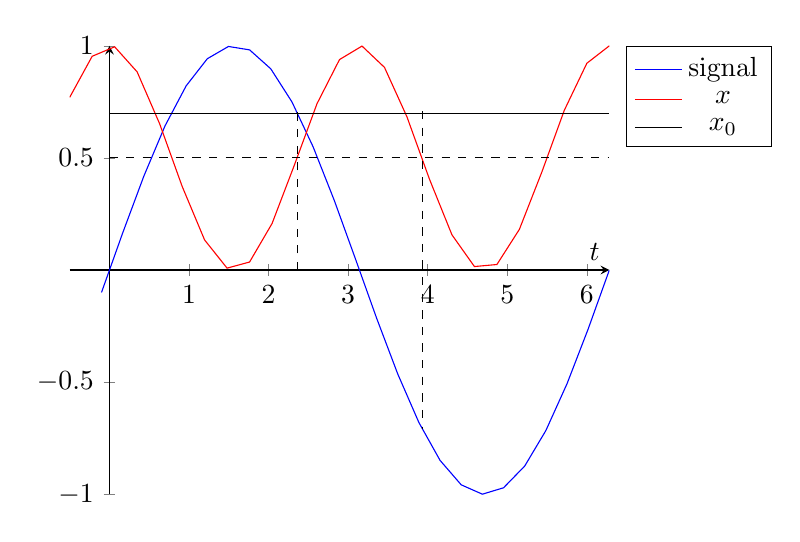
\begin{tikzpicture}
		\begin{axis}[axis lines=center, xlabel=$t$, domain=-.5:2*pi, legend pos=outer north east]
		\addplot[color=blue, name path=signal, domain=-.1:2*pi] {sin(deg(x))}; \addlegendentry{signal}
		\addplot[color=red] {cos(deg(x))^2}; \addlegendentry{$x$}
		\addplot[mark=none, domain=0:2*pi]{.7}; \addlegendentry{$x_0$}
		\addplot[mark=none,dashed, domain=0:2*pi]{.5};
		\draw[dashed] (axis cs:2.36,0) -- (axis cs:2.36,{sin(deg(2.36))});
		\draw[dashed] (axis cs:3.93,{-sin(deg(3.93))}) -- (axis cs:3.93,{sin(deg(3.93))});
		\end{axis}
	\end{tikzpicture}
	\caption{Explanation for $x_0$\label{fig:x0Expl}}
\end{figure}

The number of events per zero-crossing 
\[
	\Nozc = \frac{\Delta t_{zc}}{\Nmo\cdot \Delta t_{\meas}},
\]
hence
\[
	X_{tot} = g(\Nzc) \cdot \frac{\Delta t_{zc}}{\Delta t_{\meas}}\cdot \frac{1}{\Nmo}.
\]

The variance $\var[w]{t}$ is also practically independent of how many measurements there are per one zero-crossing (and by extension, the number $\Nmo$), and depends primarily on the $\Nzc$ and decoherence life time.

In sum, assuming one observation is the mean of the measurements ($\SE{\obs} = \SE{\meas}/\sqrt{\Nmo}$), 
\begin{align*}
	\var[w]{\hat{\omega}} &= \frac{\SE{\meas}^2\cdot \sfrac{1}{\Nmo}}{g(\Nzc)\cdot \frac{\Delta t_{zc}}{\Delta t_{\meas}}\cdot \sfrac{1}{\Nmo} \cdot \var[w]{t}} \\
		&= \frac{\SE{\meas}^2}{g(\Nzc)\cdot \frac{\Delta t_{zc}}{\Delta t_{\meas}} \cdot \var[w]{t}}
\end{align*}


\section{Spin tune decoherence time}

We have the Cram\'er-Rao inequality to tell us what's the minimum variance of an estimator is possible:
\[
	\var{\hat{\omega}} \geq \frac{1}{\Fisher(\omega)}.
\]
Fisher information is additive, and what I call \emph{point Fisher information} can be expressed as:
\[
	\Fisher[i] = \frac{1}{\nu}\begin{pmatrix}
		\bkt{\sqrt{2}\cdot\mupp}^{-2} & 0     & 0   \\
		0                             & t_i^2 & t_i \\
		0                             & t_i   & 1
	\end{pmatrix}\cdot \bkt{\mupp}^2.
\]

\begin{wrapfigure}{l}{.25\textwidth}
	\begin{tikzpicture}
	\draw[->] (-1.5,0) -- (1.5,0) node[right] {$\mupp$};
	\draw[->] (0,-.5) -- (0, 2.3) node[above] {$I_i(\pars_0)$};
	\draw[scale=1,domain=-1.5:1.5,smooth,variable=\x,red] plot ({\x},{\x*\x});
	\end{tikzpicture}
\end{wrapfigure}





\end{document}